\chapter{Lecture 4 (1/26)}
    The fourth lecture of Physics 137B was held on \textbf{Thursday, January 26}. It covered \textbf{more on the addition of spin, as well as introducing the famous 2-electron states (singlet and triplet)}.

    \section{Last Time: Adding in Spin for Many Particles}
        Last time, we recognized that the picture of the many particles in a box that we had been working with was incomplete. Even ignoring particle-particle interactions, we were still omitting the spin component of the many-body wavefunction and considering only the orbital (spatial) component. And so, we started by giving each of the particles in our box some kind of spin:
        $$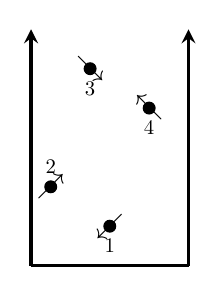
\begin{tikzpicture}
            \draw[very thick, -stealth] (0,0) -- (0,3);
            \draw[very thick, -stealth] (2,0) -- (2,3);
            \draw[very thick] (0,0) -- (2,0);

            \filldraw[black] (0.25,1) circle (0.075cm);
            \filldraw[black] (1,0.5) circle (0.075cm);
            \filldraw[black] (0.75,2.5) circle (0.075cm);
            \filldraw[black] (1.5,2) circle (0.075cm);
            \node[scale=0.75] at (1,0.25) (i) {$1$};
            \node[scale=0.75] at (0.25,1.25) (ii) {$2$};
            \node[scale=0.75] at (0.75,2.25) (iii) {$3$};
            \node[scale=0.75] at (1.5,1.75) (iv) {$4$};
            \node at (0.25,1) (ne) {$\nearrow$};
            \node at (1,0.5) (sw) {$\swarrow$};
            \node at (0.75,2.5) (se) {$\searrow$};
            \node at (1.5,2) (nw) {$\nwarrow$};
        \end{tikzpicture}$$
        Now, we stated how the orbital part of our wavefunction told us only about the \textit{location} of each particle in space, but now we also factor in the \textbf{spin} part, which will tell us about the \textit{spin angular momentum}. The simplest combination is simply the product state:
        $$\Psi_{\mathrm{MB}} = \left(\Psi_{\mathrm{MB}}^{\mathrm{orbit}}\right)\left(\Psi_{\mathrm{MB}}^{\mathrm{spin}}\right)$$
        Similarly, the simplest way to get our many-body spin state is also to take a product state of each single-particle spin state:
        $$\Psi_{\mathrm{MB}}^{\mathrm{spin}} = \ket{s_1\ m_1}\ket{s_2\ m_2}\dots\ket{s_N\ m_N}$$
        For simplicity, we'll deal with electrons for now, which have spin-$\frac12$ (in other words, $s = \frac12$). This means that $m = \pm\frac12$, meaning that the total number of product states is $2^N$, where $N$ is the number of particles in our box.\\\\
        As we found out last time, it turns out that each of these product states is an eigenstates of each of the operators $(\hat{S}_1^2, \hat{S}_{1_Z}), (\hat{S}_2^2, \hat{S}_{2_Z}), \dots, (\hat{S}_N^2, \hat{S}_{N_Z})$. Now, this product basis is fairly intuitive to deal with, but it might not always be the most helpful, which is why we were interested in creating a new spin basis, that we called the \textit{total spin}:
        \begin{align*}
            \hat{S}_T &= \hat{S}_1 + \hat{S}_2 + \dots + \hat{S}_N\\
            \hat{S}_T^2 &= \hat{S}_T\cdot\hat{S}_T\\
            \hat{S}_{T_Z} &= \hat{S}_{1_Z} + \hat{S}_{2_Z} + \dots + \hat{S}_{N_Z}
        \end{align*}
        In other words, total spin converts our system from eigenstates of $(\hat{S}_1^2, \hat{S}_{1_Z}), (\hat{S}_2^2, \hat{S}_{2_Z}), \dots, (\hat{S}_N^2, \hat{S}_{N_Z})$ into just eigenstates of $(\hat{S}_T, \hat{S}_Z)$\footnote{I may sometimes omit the hats when writing these operators, but whenever we're dealing with them, it's implied that the hats are there.}.\\\\
        So, how do we convert to this?
    \section{Continuing Addition of Spin}
        Well, last semester (or whenever you took 137A), we learned about the properties of the $S^2$ and $S_Z$ operators for single particles. So, naturally, we want our commutator relations for the total spin operators to match up\footnote{It seems pretty logical that our commutation relations should work this way, and we can prove it ourselves (but we won't do that here).}:
        \begin{theorem}{Commutation Relations for Total Spin Operators}{}
            $$[\hat{S}_T^2,\hat{S}_{T_Z}] = 0, \ \ \ [\hat{S}_{T_i},\hat{S}_{T_j}] = i\hbar\hat{S}_{T_k} \ \ \scriptstyle(i,j,k) = (x,y,z)$$
        \end{theorem}
        In other words, the algebra for these operators will be the same as the algebra that we had for our single-particle spin operators last semester.
        \begin{insight*}{}{}
            Properties of operators lie inside the commutator. In other words, once we have commutator relations, we can derive everything about an operator. This is super important.
        \end{insight*}
        So, now we can find the eigenstates, assuming the algebra works out the same way:
        \begin{align*}
            \hat{S}_T^2\ket{s_T \ m_T} &= \hbar^2s_T(s_T+1)\ket{s_T\ m_T}\\
            \hat{S}_{T_Z}\ket{s_T\ m_T} &= \hbar m_T\ket{s_T\ m_T}
        \end{align*}
        \subsection{Total Raising and Lowering Operators}
            We can derive these relations by defining our raising and lower operators and doing the same thing as we've done before for the single particle cases:
            \begin{definition}{Total Raising and Lowering Operators}{}
                Denoted $\hat{S}_{T_+}$ and $\hat{S}_{T_{-}}$, respectively: $$\fbox{$\hat{S}_{T_{\pm}} = \hat{S}_{T_x} \pm i\hat{S}_{T_y}$}$$
            \end{definition}
            So, we then see how these act on our spin states:
            $$\hat{S}_{T_{\pm}}\ket{s_T, m_T} = \hbar\sqrt{s_T(s_T+1)-m_T(m_T\pm 1)}\ket{s_T, m_T\pm 1}\footnote{I may sometimes put commas to separate the quantum numbers in the spin states, but it means the same thing as when there's no comma separation.}$$
            Now, since we're dealing with $s = \frac12$, we can simplify our notation a little bit:
            \begin{notation*}{}{}
                For $s=\frac12$, \fbox{$\ket{\frac12,\frac12} = \ket{\ua}$}, \fbox{$\ket{\frac12,-\frac12} = \ket{\da}$}
            \end{notation*}
        \subsection{Finding Eigenstates}
            Now, we're about to try to find $\ket{s_T,m_T}$, but what does it mean to do that? Well, we know the product states:
            $$\Psi^{\mathrm{Prod}} = \ket{m_1,m_2,\dots,m_N}\footnote{Since we're dealing with $s=\frac12$, we'll omit $s$ from our notation entirely for now.}$$
            So, now a question:
            $$\fbox{Is the product states $\Psi^{\mathrm{Prod}}$ an eigenstate of $\hat{S}_{T_Z}$?}$$
            To answer this, we simple take $\hat{S}_{T_Z}$ and act it on $\Psi^{\mathrm{Prod}}$:
            $$\hat{S}_{T_Z}\Psi^{\mathrm{Prod}} = \lambda\Psi^{\mathrm{Prod}}$$
            Here, $\lambda$ is some constant eigenvalue. Let's see if we can even do that by expanding out $\hat{S}_{T_Z}$:
            $$(\hat{S}_{1_Z}+\hat{S}_{2_Z}+\dots+\hat{S}_{N_Z})\ket{m_1,m_2,\dots,m_N} = \underbrace{\hbar(m_1+m_2+\dots+m_N)}_{\text{eigenvalue!}}\ket{m_1,m_2,\dots,m_N}$$
            Wait, where did all of that come from? The key insight here is that each individual single-particle spin operator will only act on the corresponding single-particle spin state! So, we simply get a big sum, and thus it \fbox{is} an eigenstate!
            \begin{remark*}{}{}
                The product state, for this reason among others, is a great, useful, and \underline{easy} basis to work with.
            \end{remark*}
            So, we've confirmed that this big state is an eigenstate of $\hat{S}_{T_Z}$, \underline{but is it an eigenstate of $\hat{S}_T^2$}?
            $$\fbox{As it turns out, sometimes yes, and sometimes no.}$$
            This leads us back to our original question: \underline{how do we get to our eigenstates $\ket{s_T,m_T}$}?\\\\
            The first clarifying question we should ask when presented with this problem is:
            $$\fbox{What basis are we working in?}$$
            This is because our answer will depend on the basis. Well, what's the easiest base to work in? The product basis, of course! So, we need to construct the eigenstates of $S_{T}^2$ out of the product basis. How do we do this? Well, as is the case with most linear algebra problems, the solution is fairly simple: \underline{construct a matrix and diagonalize it}!\\\\
            Recall how to find matrix entries from 137A:
            \begin{theorem}{Matrix of an Operator Revisited}{}
                $$S_{T_{ij}}^2 = \bra{i}\hat{S}_{T}^2\ket{j}$$
            \end{theorem}
            In the case of our product basis, the $i$s and $j$s are our product states! So, our matrix will be $2^N\times2^N$ and look like this:
            $$\hat{S}^2 = \begin{pmatrix}S_{11}^2 & S_{12}^2 &\dots & & \\ S_{21}^2 & S_{22}^2 & \dots & & \\ \vdots & & \ddots & & \\ & & & & & \\ & & & & &\end{pmatrix}$$
            So, properly diagonalizing this matrix will give us the eigenstates along the diagonal.
            \subsubsection{We Hate Diagonalizing Matrices}
                There's just one slight caveat: \underline{nobody wants to do this}. The matrix gets really big really quickly, so diagonalizing it is, while correct, an extremely tedious process. Naturally, the motto of this class is then as follows:
                $$\fbox{We hate this. Avoid this massive matrix stuff at all costs.}$$
                So, what are we going to do instead? Well, to illustrate, let's do a simple example. Let's find the total angular momentum states for two electrons:
                \begin{example}{Total Angular Momentum States for Two Electrons}{}
                    Consider our box again:
                    $$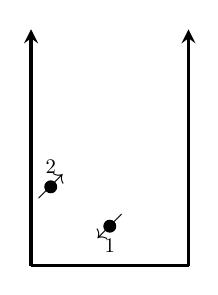
\begin{tikzpicture}
                        \draw[very thick, -stealth] (0,0) -- (0,3);
                        \draw[very thick, -stealth] (2,0) -- (2,3);
                        \draw[very thick] (0,0) -- (2,0);
            
                        \filldraw[black] (0.25,1) circle (0.075cm);
                        \filldraw[black] (1,0.5) circle (0.075cm);
                        \node[scale=0.75] at (1,0.25) (i) {$1$};
                        \node[scale=0.75] at (0.25,1.25) (ii) {$2$};
                        \node at (0.25,1) (ne) {$\nearrow$};
                        \node at (1,0.5) (sw) {$\swarrow$};
                    \end{tikzpicture}$$
                    Again, what are the eigenstates of $S_T^2$ and $S_{T_Z}$? Well, it's not too ba din this example, since we only have a $4\times4$ matrix. Let's first figure out the product basis (there are 4 states):
                    $$\Psi_{\mathrm{MB}}^{\mathrm{Spin}} = \ket{s_1 \ m_1}\ket{s_2 \ m_2}$$
                    We hate this notation, though, so let's simplify it:
                    \begin{align*}
                        \ket{\ua}_1\ket{\ua}_2 &= \ket{\uu} = \ket{\frac12,\frac12}\\
                        \ket{\ua}_1\ket{\da}_2 &= \ket{\ud} = \ket{\frac12,-\frac12}\\
                        \ket{\da}_1\ket{\ua}_2 &= \ket{\du} = \ket{-\frac12,\frac12}\\
                        \ket{\da}_1\ket{\da}_2 &= \ket{\dd} = \ket{-\frac12,\frac12}
                    \end{align*}
                    What now? In principle, we would go about diagonalizing the resultant $t4\times4$ matrix. But, that already gets clunky, so let's not do that. This is a linear agebra problem, but this is a physics class, so let's instead use some clever linear algebra reasoning to avoid diagonalizing a matrix, since, remember, we don't like doing that.\\\\
                    Consider those states again. How do we find $m_T$ for each of them? Simple: just add $m_1+m_2$:
                    \begin{align*}
                        \ket{\uu} &\implies m_T = 1\\
                        \ket{\ud} &\implies m_T = 0\\
                        \ket{\du} &\implies m_T = 0\\
                        \ket{\dd} &\implies m_T = -1
                    \end{align*}
                    Cool. Now, are these eigenstates of $S_T^2$ and $S_{T_Z}$? Yes! So, we now need to find $s_T$ for each of them. Let's be clever about this. Starting with some product state (say, for simplicity, $\ket{\uu}$), what should $s_T$ be?\\\\
                    Well, we know that for a given $s_T$, $m_T$ will range from $-s_T$ to $s_T$ and will increment by $1$ each time. So, that means that, if $m_T = 1$, then $s_T \neq 0$ right off the bat. Cool. Can it be $2$? Well, technically, this condition is no longer violated, but if $s_T$ were equal to $2$, that would mean that we'd need to have some state in our basis with $m_T = 2$ and $m_T = -2$ (since our basis is complete and spans the entire Hilbert space), which we don't have. Thus, $s_T$ can't be $2$. Is there a happy medium between $0$ and $2$? For anyone that's passed Kindergarten, the answer is $1$. So, \fbox{$s_T = 1$}.\\\\
                    We did a lot of handwavy stuff, so let's prove it:
                    \begin{multline*}
                        S_T^2\ket{\uu} = (\hat{S}_1 + \hat{S}_2)\cdot(\hat{S}_1+\hat{S}_2)\ket{\uu} = (\hat{S}_1^2+\hat{S}_2^2+2\hat{S}_1\cdot\hat{S}_2)\ket{\uu} = \\
                        = [\hat{S}_1^2+\hat{S}_2^2+2(S_{1x}S_{2x}+S_{1y}S_{2y}+S_{1z}S_{2z})]\ket{\uu}
                    \end{multline*}
                    Now, we know:
                    \begin{align*}
                        \hat{S}_1^2\ket{\uu} &= \hbar^2\left(\frac12*\frac32\right)\ket{\uu} &&\text{(Only acts on the first arrow!)}\\
                        \hat{S}_{1z}\ket{\uu} &= \frac{\hbar}{2}\ket{\uu}
                    \end{align*}
                    So, those are easy. What about $S_{1x}S_{2x}$ and $S_{1y}S_{2y}$? Use the raising and lowering operators!
                    \begin{definition}{Rewriting Ladder Operators}{}
                        \fbox{$\hat{S}_x = \frac12(\hat{S}_+ + \hat{S}_-)$}, \fbox{$\hat{S}_y = \frac{1}{2i}(\hat{S}_+ - \hat{S}_-)$}
                    \end{definition}
                    So, for spin $\frac12$, we have that $S_+\ket{\da} = \hbar\ket{\ua}$ and $S_-\ket{\ua}=\hbar\ket{\da}$. Now, we can grind through this math (we'll skip it here, but in principle it wouldn't be too hard to execute). After all of the work:
                    $$\hat{S}_T^2\ket{\uu} = \hbar^2*(1*(1+1))\ket{\uu} = \hbar^2s_T(s_T+1)\ket{\uu}$$
                    Thus, the math works out for $s_T = 1$, as desired. $\blacksquare$\\\\
                    So, we've confirmed $s_T=1$ for our first case. This means our first eigenstate is:
                    $$\fbox{$\ket{s_T\ m_T} = \ket{1,1} = \ket{\uu}$}$$
                    The middle expression is our new basis, and the last one is the new expression in terms of the old basis. Let's now keep going. We now need to find out what the other three eigenstates are. So, let's go to the next state ($m_T = 0$) by simply acting the lowering operator on our highest state $\ket{1,1}$:
                    $$\ket{1,0} = A\hat{S}_{T_-}\ket{1,1} = A\hat{S}_{T_-}\ket{\uu}$$
                    Here, we want to isolate the constant $A$. Let's act $\hat{S}_{T_x} - i\hat{S}_{T_y}$ on $\ket{\uu}$ to find it:
                    $$\hat{S}_{T_-}\ket{\uu} = (\hat{S}_{T_x} - i\hat{S}_{T_y})\ket{\uu} = \underbrace{[(\hat{S}_{1x} + \hat{S}_{2x}) - i(\hat{S}_{1y}+\hat{S}_{2y})]}_{\text{Plug in desired values here}}\ket{\uu}$$
                    Skipping ove rthe fussy algebra, we end up with:
                    $$\fbox{$\hat{S}_{T_-} = \hat{S}_{1_-} + \hat{S}_{2_-}$} \implies \hat{S}_{T_-}\ket{\uu} = \hbar(\ket{\du} + \ket{\ud})$$
                    Remember, each of the single-particle lowering operators will act on the corresponding single state. So, putting it together:
                    $$\ket{1,0} = A(\ket{\du} + \ket{\ud}) \implies \overbrace{\braket{1,0} = 1}^{\text{Isolate $A$ like this}} \implies \fbox{$A = \frac{1}{\sqrt2}$}$$
                    Thus, we end up with:
                    $$\fbox{$\ket{1,0} = \frac{1}{\sqrt2}(\ket{\du} + \ket{\ud})$} \implies \fbox{$s_T = 0$}$$
                    Next, how do we get to $\ket{1,-1}$? Lower again!
                    $$\ket{1,-1} = S_{T_-}\ket{1,0} = (\hat{S}_{1_-} + \hat{S}_{2_-})\frac{1}{\sqrt2}(\ket{\du} + \ket{\ud}) = \text{...some painful algebra...} \ket{\dd}$$
                    Thus, we have:
                    $$\fbox{$\ket{1,-1} = \ket{\dd}$} \implies \fbox{$s_T = 1$}$$
                    So, all that we're missing is $s_T = 0$. We get this from $\ket{0,0}$. Now, how do we get this? Well, are all of these states orthogonal? Yes! Why? They're all eigenstates of a hermition operator $\hat{S}_T^2$. So, this means that $\ket{0,0}$ must be orthogonal to $\ket{1,0}$, which means we have our final eigenstate as well:
                    $$\fbox{$\ket{0,0} = \frac{1}{\sqrt2}(\ket{\ud} - \ket{\du})$} \implies \fbox{$s_T = 0$}$$
                    You can show that these two states are orthogonal by taking their inner product and confirming that it is indeed equal to $0$:
                    $$\braket{1,0}{0,0} = \frac12(\bra{\ud}+\bra{\du})(\ket{\ud}-\ket{\du}) = \frac12\left(\braket{\ud}{\du} - \braket{\ud}{\du} - \dots\right) = \fbox{$0$} \ \ \checkmark$$
                    And so, we have all of the eigenstates! We could've done this the brute force way with matrix diagonalization, but this reasoning more than suffices for giving us our desired eigenstates.
                \end{example}
                That was quite a long example, but it illustrates how powerful this \say{quick} linear algebra reasoning is. While the matrix diagonalization may not take too much time with a $4\times4$ matrix, the time it would take grows exponentially the more product states we add, and this linear algebra reasoning will help us get these results much quicker.
    \section{The Singlet And The Triplet}
        This result that we derived in the precious example is big and quite useful, since we now have our desired eigenstates for two electrons.
        \begin{insight*}{}{}
            These particular results are quite handy and we derived them because they are used quite a lot in physics.
        \end{insight*}
        So, to summarize, we found the total spin eigenstates for two identical spin-$\frac12$ particles (namely electrons), which have some very special (and familiar) names:
        \begin{theorem}{Singlet and Triplet States}{}
            \begin{align*}
                \textbf{Triplet States}: s_T = 1 &\implies \fbox{$\begin{cases}\ket{1,1} = \ket{\uu} & m_T = 1\\ \ket{1,0} = \frac{1}{\sqrt2}(\ket{\ud} + \ket{\du}) & m_T = 0\\ \ket{1,-1} = \ket{\dd} & m_T = -1\end{cases}$}\\
                \textbf{Singlet State}: s_T = 0 &\implies \fbox{$\ket{0,0} = \frac{1}{\sqrt2}(\ket{\ud}-\ket{\du})$, $m_T = 0$}
            \end{align*}
        \end{theorem}
        As we can see, we now have a better understanding of where the terms \say{triplet} and \say{singlet} come from: \textit{they come from the total spin number }$s_T$!
        \subsection{A Generalization}
            Now, let's generalize what we've done, since therte's an important pattern for adding angular momentum that we wish to make explicit here.\\\\
            We took the product basis $s_1 = \frac12 \otimes s_2 = \frac12$ and we converted it to the total spin basis. Now, in the product basis, there were $2\times2=4$ possible states, and in our new total spin basis, there are $3+1=4$ possible states as well. It makes sense that the number of states hasn't changed, but now we want to make explicit how exactly it does.
            \begin{theorem}{Generalizing Total Spin States For 2 Particles}{}
                Suppose we have two spins, $s_1$ and $s_2$. Then, the total spin becomes $s_T$, which can range from $s_1+s_2$ up to $|s_1 - s_2|$ (it needs to be nonnegative).
            \end{theorem}
            \begin{remark*}{}{}
                We could see this pattern in our special case already.
            \end{remark*}
            Now, to prove this fact that we stated, we could in principle use inductive reasoning, but because this isn't a math class, we'll skip over that and take it as true. Let's consider a basic example to illustrate our new rule:
            \begin{example}{$\mathbf{s_1 = 1}$, $\mathbf{s_2 = 3}$}{}
                In this case, we can construct the product states first. $s_1$ has 3 associated states ($1,0,-1$), and $s_2$ has 7 ($3,2,1,0,-1,-2,-3$). So, in total, we have $3\times 7 = \fbox{$21$}$ total product states.\\\\
                Now, adding them together to get the total spin, we see that $s_T$ can take on values $4,3,2$ (since that's $|s_1 - s_2|$). Now, for $s_T = 4$, we have $9$ states (using the same logic as we did for the individual states). Similarly, for $s_T=3$, we have $7$ states, and for $s_T=2$, we have $5$. Putting it together, we have $9+7+5=\fbox{$21$}$ possible total states here as well, which exactly equals what we had in the product basis. So, it works!
            \end{example}
        \subsection{Symmetry of The Triplet And Singlet}
            Let's look at one other cute thing. Let's consider the symmetry of these total angular momentum states (triplet and singlet). To do that, let's act the exchange operator on our states:
            \begin{align*}
                \hat{P}_{12}\ket{1,1} &= \ket{11} &&\text{\underline{symmetric}}\\
                \hat{P}_{12}\ket{1,0} &= \frac{1}{\sqrt2}(\ket{\du}+\ket{\ud}) &&\text{\underline{symmetric}}\\
                \hat{P}_{12}\ket{1,-1} &= \ket{\dd} &&\text{\underline{symmetric}}\\
                \hat{P}_{12}\ket{0,0} &= \frac{1}{\sqrt2}(\ket{\du}-\ket{\ud}) &&\text{\underline{antisymmetric}}
            \end{align*}
            So, we see the following:
            $$\fbox{Triplets are symmetric, but the singlet is antisymmetric!}$$
            Let's apply this to two particles (electrons) in a box.
            \subsubsection{Ground State of Two Electrons in a Box}
                If we want to construct a proper state in the box, how do we put them into the box? Well, let's first put them in the ground state to see what our state should look like then:
                $$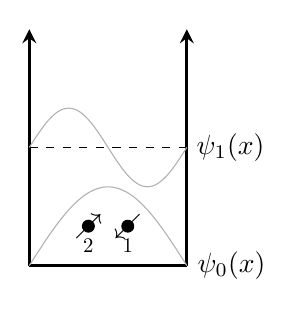
\begin{tikzpicture}
                    \draw[very thick, -stealth] (0,0) -- (0,3);
                    \draw[very thick, -stealth] (2,0) -- (2,3);
                    \draw[dashed] (0,1.5) -- (2,1.5) node[anchor=west] {$\psi_1(x)$};
                    \draw[very thick] (0,0) -- (2,0) node[anchor=west] {$\psi_0(x)$};
        
                    \filldraw[black] (0.75,0.5) circle (0.075cm);
                    \filldraw[black] (1.25,0.5) circle (0.075cm);
                    \node[scale=0.75] at (1.25,0.25) (i) {$1$};
                    \node[scale=0.75] at (0.75,0.25) (ii) {$2$};
                    \node at (0.75,0.5) (ne) {$\nearrow$};
                    \node at (1.25,0.5) (sw) {$\swarrow$};
                    \draw[thin,gray!60] (0,0) sin (1,1) cos (2,0);
                    \draw[thin,gray!60] (0,1.5) sin (0.5,2) cos (1,1.5) sin (1.5,1) cos (2,1.5);
                \end{tikzpicture}$$
                Our wavefunction then becomes:
                $$\Psi_{\mathrm{MB}} = \left(\Psi_{\mathrm{MB}}^{\mathrm{orbit}}\right)\left(\Psi_{\mathrm{MB}}^{\mathrm{spin}}\right) = (\psi_0(x_1)\psi_0(x_2))\underbrace{\left(\frac{1}{\sqrt2}(\ket{\ud - \ket{\du}})\right)}_{\text{has to be antisymmetric!}}$$
                Notice that our overall wavefunction needs to be \textit{antisymmetric}, and our orbital component here is symmetric (since that's the only possible one), which means consequently that our spin component must be antisymmetric. Thus, we only have one possible expression for the total spin, illustrated above.\\\\
                And that's our ground state!
                \begin{insight*}{}{}
                    This is what covalent bonds look like! This is what their wavefunction has to look like, since this is the only way the math and the physics can work out! They're always singlets!
                \end{insight*}
                These bonds are also entangled and have a lot of other interesting properties, but more on that next time!
